\section{Neural Radiance Fields~--~NeRFs}\label{NeRF}

Neural Radiance Fields (NeRFs), as introduced by \citeauthor{mildenhallNERF}, offer a groundbreaking approach to representing 3D scenes from a limited set of 2D images \citep{mildenhallNERF}. Unlike conventional 3D reconstruction methods, which often have problems capturing complex geometries and variable lighting conditions, NeRFs use a volumetric representation to accurately capture both the spatial and angular distribution of light. This is achieved by modeling the volumetric scene as a continuous 5D function, accepting 3D spatial coordinates and viewing direction as inputs, and generating the color and opacity at a given point in the scene as outputs. This fundamental change in representation allows NeRFs to address challenges common to traditional techniques and provide a more robust framework for reconstructing and rendering 3D scenes \citep{mildenhallNERF}.

\begin{figure}[ht]
    \centering
      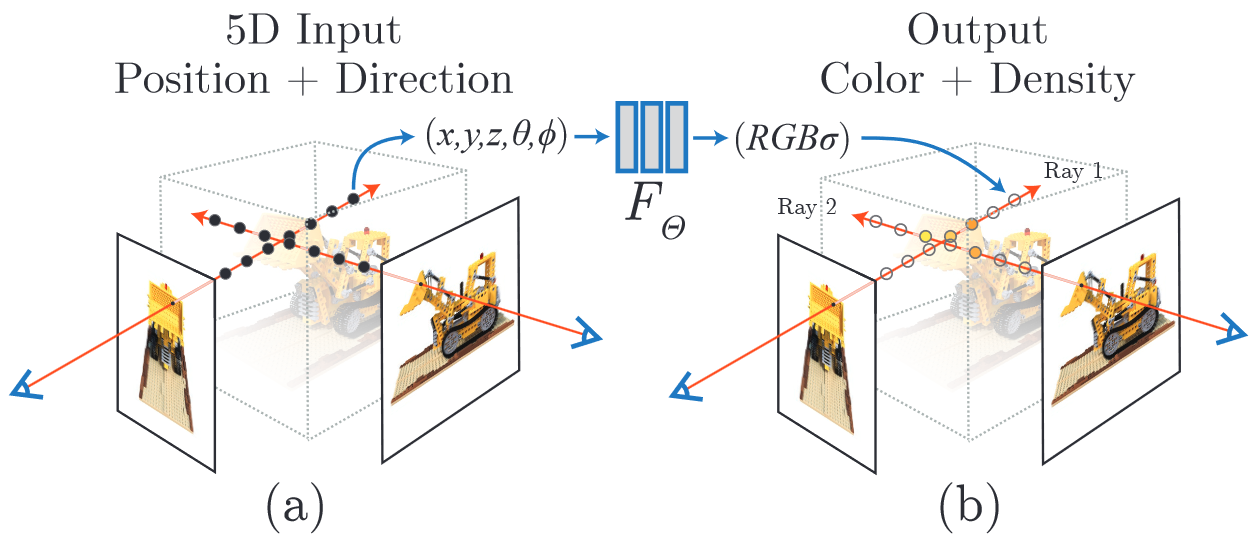
\includegraphics[width=1\columnwidth]{figures/NeRF_Fig_2_Mildenhall.png}
      \caption{Neuronal Radiance Field. Figure taken From Mildenhall~\cite{mildenhallNERF}~--~Figure 2}\label{fig:figureNeRF}
\end{figure}


Classic deep learning methods often require a comprehensive dataset comprising various scenes and their representations. NeRFs, on the other hand, are trained to specialize in a single, unique scene \citep{mildenhallNERF}. The underlying neural network consists of Fully Connected Layers (FCs) with ReLU activations, specifically designed to encode the volumetric details of that particular scene, effectively creating a dedicated neural network for each scene \citep{mildenhallNERF}. The neural network accepts two types of input: a position in a given coordinate system, often expressed as a 3D vector \(x, y, z\), and a viewing direction represented by two angles \( \theta, \phi \). To better understand the concept of the latter two inputs, imagine a scenario where a flashlight is held in the middle of a dark room. The angle \( \theta \) would represent how much the flashlight is tilted up or down. Similarly, the angle \( \phi \) would represent how much the flashlight is rotated about the vertical axis while pointed outward. These angles help the neural network understand from which direction the beam is being cast to a point in 3D space. The network's output consists of the color \(c\) and density \( \sigma \) at that particular location \citep{mildenhallNERF}. Queries to the neural network can be made by projecting a ray through the scene and asking for color and density information at various points along the ray. This unique querying process enables capturing complex visual phenomena like lighting, reflections, and transparency, which are often challenging to model with traditional 3D reconstruction techniques. For each pixel in a desired image frame, the neural network is queried at multiple points along a ray projected through the scene to produce a curve representing the density of objects along the ray's path, as seen in part (c) of Figure~\ref{fig:figureNeRF}. The point at which this density curve rises significantly usually corresponds to an object in the scene, and the color at this point is what is rendered for that particular pixel. These density and color curves can be visualized using graphs to illustrate how density and color vary along the ray's path. For instance, if a ray intersects a tree, the density would increase and the color output would likely be green, representing the tree's leaves \citep{mildenhallNERF}.

The network can also handle multi-view consistency, predicting color as a function of both location and viewing direction, while density is predicted solely based on location. This distinction is grounded in the idea that density, or transparency, is invariant to the direction from which an object is viewed \citep{hu2023consistentnerf}. Therefore, to generate the color, the model first computes the density and a hidden representation based on the location. This hidden representation is then concatenated with the viewing direction and passed through another set of layers to produce the color.

An integral aspect of setting up NeRFs involves solving the problem of identifying the camera's position and direction for each input image. Methods like Structure-from-Motion (SfM) and Simultaneous Localization and Mapping (SLAM) can address this issue \citep{wei2021nerfingmvs}. Once these parameters are identified, new views can be synthesized by querying the neural network for color and density information along rays projected through the scene \citep{gerats2023dynamic}. Another challenge arises during training due to the absence of explicit density information. Nevertheless, the training process can be managed by minimizing the loss between predicted and observed values from input images. The model employs backpropagation, as its entire pipeline for rendering images, which includes casting rays, sampling along these rays, and integrating the sampled values to compute a pixel's color, is differentiable \citep{yariv2020multiview}.

In Neural Radiance Fields (NeRF), volume rendering with radiance fields employs the formula 

\[ 
C(r) = \int_{t_n}^{t_f} T(t)\sigma(r(t))c(r(t), d)dt \quad \text{where} \quad T(t) = \exp\left(-\int_{t_n}^t \sigma(r(s))ds\right) 
\]

This formula \citep{mildenhallNERF} facilitates the rendering of a 3D scene by casting rays and aggregating their properties from a near boundary (\(t_n\)) to a far boundary (\(t_f\)). In simpler terms, as a ray traverses through the scene, this formula accumulates color information based on the density and transparency of objects along the ray's path. Specifically, \( T(t) \) quantifies the transparency of the scene at a particular point along the ray, denoting how much light penetrates through, while \( \sigma(r(t)) \) denotes the density of objects at a particular point along the ray, with higher density implying more matter at that point. The term \( c(r(t), d) \) denotes the color at a particular point along the ray, given the viewing direction \( d \). This calculation determines whether the ray continues through empty space or ends when it hits an object, with color adjustments made at this endpoint \citep{mildenhallNERF}.

Although naive NeRF models may not provide photorealistic results due to the lack of detail, several optimizations have been introduced to improve their performance. One notable improvement is the use of positional encoding techniques that deterministically map 3D coordinates and view directions to a higher dimensional space. This is achieved by using high-frequency features before inputting them to the multilayer perceptron (MLP), which helps optimize the neural radiation fields to better represent high-frequency scene content \citep{mildenhallNERF}. Hierarchical volume sampling is another important optimization. This strategy involves two neural network systems, one coarse and one refined, which are jointly optimized during training. Initially, the coarse network sparsely samples the rays in the 3D scene, and based on this initial sampling, the refined or ``fine'' network is guided to perform a more detailed sampling. This hierarchical approach is critical because dense sampling is very computationally expensive. A two-tier system therefore helps manage computational resources while allowing detailed sampling along rays to obtain the density and color of the sampled points \citep{arandjelović2021nerf}.

The experimental results highlight several notable strengths and limitations of the Neural Radiance Fields (NeRF) approach. One of its key advantages is the model's ability to represent fine-grained structures. Another advantage of NeRF is its memory efficiency. For example, rendering a single scene with NeRF requires only about five megabytes of memory, which is in stark contrast to voxel grid renderings that require over 15 gigabytes for a comparable scene \citep{mildenhallNERF}. This mismatch in memory requirements underscores NeRF's superior efficiency in terms of data storage and transfer, and represents a compelling advantage over traditional 3D rendering techniques \citep{mildenhallNERF}. Remarkably, the memory requirement of the rendered scene is even smaller than that of the input images, making the model extremely efficient in data storage and transfer \citep{mildenhallNERF}.
However, the NeRF model is not free of limitations. A major challenge is the computational cost associated with training the neural network. The optimization process for a single scene may require about 100,000 to 300,000 iterations to converge, assuming the use of a single NVIDIA V100 GPU \citep{mildenhallNERF}. This is equivalent to a training period of about one to two days. While this does not require a data center, it does require a significant amount of time, making NeRF less suitable for scenarios that require rapid implementation. In addition, NeRF rendering is prone to sampling and aliasing issues that can lead to significant artifacts in the synthesized images \citep{rabby2023beyondpixels}. These artifacts arise from the limited sampling of the radiation field, resulting in inaccurate reconstruction of certain features, especially in scenes containing sharp edges or textures \citep{rabby2023beyondpixels}. The slow training speed and rendering, especially at high resolutions, further exacerbate the problems, making NeRF impractical for real-time applications or for generating animations that span multiple frames \citep{rabby2023beyondpixels}.

\textcolor{blue}{One of the notable strengths of NeRFs lies in their capability for view-dependent appearance modeling. The system considers how the appearance of an object or scene varies with the direction from which it is viewed, offering a more nuanced and realistic visual impression. This view-dependent feature of NeRFs enables the synthesis of images that accurately reflect how differently the same scene or object can appear when viewed from different angles. In addition, NeRFs offer the ability to capture more complicated geometries and occlusions. The method is capable of producing detailed depth maps that are often difficult to obtain using traditional techniques, especially for complex scenes. These depth maps are versatile enough to support mixed reality applications and allow seamless integration of virtual objects into real-world environments. The system also facilitates the conversion of Neural Radiance Fields into 3D mesh structures using marching cubes, further increasing their usefulness. Another advantage of using NeRFs is their ability to process real-world objects captured through inward-looking 360-degree views. Unlike many other methods, NeRFs do not require background isolation or masking, making them suitable for a wide range of applications. They can synthesize any intermediate view between captured images, providing a complete and flexible representation of the object or scene.
https://www.matthewtancik.com/nerf}